\begin{quote}
	``有两种推广.一种没有什么价值, 另一种则是有价值的.没什么思想、仅凭唬人的专人术语做推广是很容易做到的.颇为困难的是从若干好的素材中提取出一份精致凝练的精品.''
	\hfill ---- George Polya
\end{quote}

\section{问题的提出: 为什么要研究简单的数理逻辑}


\begin{dialogue}
	A: 问一个这一章比较简单\footnote{这里的简单并不是不用预习与听课就能自动掌握. 这里的简单指的是相对于数理逻辑这一门科目而言, 这章内容显得十分微不足道且基础.}的问题: 如果我有一个命题叫做``若$p$则$q$'', 那么这个命题的否定是什么?
	
	B: 我研究这个干什么? 闲着找事情吗? 
	
	A: 想一想你学习的极限理论. 如果我希望对于``一个数列的极限存在''这个事情做否定, 你会怎样否定? 
	
	B: 数列极限的定义是如果一个数列的极限是 $A$ , 那么就是说$\forall n>N, \exists |\epsilon|\geq 0, \text{s.t.} |a_n-A|<\epsilon$. 要是否定还是真的不是一件容易的事情啊...
	
	A: 这就是我们学习命题逻辑的原因. 以后我们会遇见成百上千的命题等待我们的操作, 如何从中找到逻辑就至关重要. 
\end{dialogue}

事实上, 很多同学是在学习数学中体会到逻辑的. 但是, 我们当中的很多人会发现: 数学仅仅是为了对付高考这样的考试. 那么希望在这一节以及以后的生活中, 慢慢体会数学带给我们的潜移默化的影响. 

这一部分我们建议参看教科书《Reading, Writing, and Proving A Closer Look at Mathematics》的第一章. 我们会在这一章主要概括一下它的主要意思. 由于是为了本科生写的数学课本, 所以句子十分的容易懂. 就当做一个小练习吧. 

\begin{prob}
	结合自己的数学学习经历, 阅读《Reading, Writing, and Proving A Closer Look at Mathematics》的第一章, 然后与下文进行比对. 看一看自己的英语理解能力如何. 不设置时间限制, 因为我们需要做的是尽可能的联系自己过去的数学学习经历, 然后去体会这段文本. 
\end{prob}


我们在生活中经常看到这样的对话: 
\begin{dialogue}
	学那么多的数学有什么用? 买菜又用不到这样的数学, 学这些还有用吗? 
\end{dialogue}

再后来, 我们发现所有的数学问题都可以通过一种``程序化''的手段来解决. 比如, 我们在上一学期学习的Gram-Schmidt正交化矩阵向量的基、解其次线性方程组、求导数等等这样的操作, 都有一系列的明确的步骤. 

那么数学仅仅是局限于此吗? 我们来看一看那些伟大的数学家的思想是什么样的: 

伟大的数学家、教育学家George Polya专门出了一本书叫做``如何解题''. 于是, 学习数学一个很重要的目的可能就是教会我们:

(1) 如何解决一个问题;

(2) 为什么这样做是对的;

(3) 这个方法什么时候是对的. 

\begin{example}
	我们是如何解含有未知数的等式(通常叫为方程), 其中一个比较重要的方法是消去律. 
	
	对于实数构成的方程, 消去律大多数都是成立的(只要等式两端不除以0), 但是对于含有未知矩阵的方程, 这样的方法很多时候就不灵了. 
\end{example}

在我们遇到一个难以解答的数学问题的时候, 还是回过头来看看George Polya为我们总结的How to solve it的一个list吧. 

\begin{pas}
\begin{center}
		\large \textbf{How to Solve it}
	\end{center}
	\begin{center}
		Summarized text\\
		Originated from George Polya's How to solve it 
	\end{center}
	First, you have to understand the problem.
	
	"Understand the problem" is often neglected as being obvious and is not even mentioned in many mathematics classes. Yet students are often stymied in their efforts to solve it, simply because they don't understand it fully, or even in part. In order to remedy this oversight, Pólya taught teachers how to prompt each student with appropriate questions,[7] depending on the situation, such as:
	
	What are you asked to find or show?[8]
	
Can you restate the problem in your own words?

Can you think of a picture or a diagram that might help you understand the problem?

Is there enough information to enable you to find a solution?

Do you understand all the words used in stating the problem?

Do you need to ask a question to get the answer?

The teacher is to select the question with the appropriate level of difficulty for each student to ascertain if each student understands at their own level, moving up or down the list to prompt each student, until each one can respond with something constructive.

Second principle: Devise a plan:

Pólya mentions that there are many reasonable ways to solve problems.[3] The skill at choosing an appropriate strategy is best learned by solving many problems. You will find choosing a strategy increasingly easy. A partial list of strategies is included:

Guess and check, Make an orderly list, Eliminate possibilities, Use symmetry, Consider special cases, Use direct reasoning, Solve an equation

Also suggested:

Look for a pattern,Draw a picture,Solve a simpler problem,Use a model,Work backward,Use a formula, Be creative. 

Applying these rules to devise a plan takes your own skill and judgement.

Polya lays a big emphasis on the teachers' behavior. A teacher should support students with devising their own plan with a question method that goes from the most general questions to more particular questions, with the goal that the last step to having a plan is made by the student. He maintains that just showing students a plan, no matter how good it is, does not help them.

Third principle: Carry out the plan

This step is usually easier than devising the plan.[23] In general, all you need is care and patience, given that you have the necessary skills. Persist with the plan that you have chosen. If it continues not to work, discard it and choose another. Don't be misled; this is how mathematics is done, even by professionals.

Fourth principle: Review/extend

Pólya mentions that much can be gained by taking the time to reflect and look back at what you have done, what worked and what did not, and with thinking about other problems where this could be useful.[24][25] Doing this will enable you to predict what strategy to use to solve future problems, if these relate to the original problem.


\end{pas}

在解答完这些问题之后, 我们往往会感到满足. 很多时候这也是我们去学习数学的一个很重要的原因. 

\begin{dialogue}
A: 可我一点感觉开心也没有啊! 

B: 可能是把做题看得太重了. 高考的``把题目作对''的观念在大学里面就应该淡化掉了. 

A: 此话怎讲?

B: 来看一看朱富海老师的文章就知道了. 

\end{dialogue}

\begin{pas}
	\begin{center}
		\large \textbf{高中数学与大学数学}
	\end{center}
	\begin{center}
		南京大学~朱富海~~节选自数林广记微信公众号
	\end{center}
	
	美国大学的数学研究者们对于学生包括中学生的培养的确非常有热情, 比如一些名校的博士生在暑假期间常常有打工的机会, 主要任务是指导一些高中生尝试做科研. 2011 年, MIT 的 Pavel Etingof 教授与另外六位作者合作出版了一本书, 题目是 Introduction to Representation Theory.
	
	这本书的内容包括代数、有限群、quiver(箭图)表示论, 以及范畴论和有限维代数结构理论, 其中的大部分内容在国内高校数学院系的本科甚至研究生课程中都讲不到. 在 Etingof 的主页可以找到这本书的 PDF 文档. 他在前言中说, 这本书是他在 2004 年给其他六位合作者的授课讲稿, 而这六位听众当时都是高中生! 其中的 Tiankai Liu 应该是华人, 在 2001, 2002, 2004 年三次代表美国队参加国际数学奥林匹克都获得金牌. 还有一位合作者是来自 South Eugene 高中的 Dmitry Vaintrob, 他在 2006 年获得面向高中生的 Siemens 竞赛的第一名, 论文题目是 The string topology BV algebra, Hochschild cohomology and the Goldman bracket on surfaces, 论文已经涉及到很深的数学理论, 在 Dmitry Vaintrob 的主页上也能找到.
	
	再看看我们在做什么? 曾经看过一道竞赛训练题, 其本质是把八位数19101112(华罗庚先生的诞生日)分解质因数. 很容易找到因数 8, 然后就一筹莫展了. 后来借助网络工具才直到 19101112 = 8×1163×2053. 看到结果有点傻眼了: 有谁能只用纸笔得到这个分解? 后来发现自己孤陋寡闻了, 有学生说这种分解质因数早就背过! 细细一想真的极为恐怖: 他们为什么要背这个? 他们又背了多少类似的东西?
	
	想想挺有意思: 杰出的数学家们用他们的智慧和汗水去探索和展现数学之美, 而我们花费了大量时间和脑细胞记忆一些很容易遗忘的意义不大的知识点, 轻轻松松地毁掉数学之美的同时顺便浇灭了学生们的求知欲.

\end{pas}

\begin{dialogue}
\begin{center}
(...对话仍在继续...)	
\end{center}
	B: 所以嘛, 我们只要把高考带来的陋习去除掉就行了. 也就是所谓的``去高考化''.
	
	A: 听起来确实很有希望. 我们终于不用再整天因为分数担惊受怕了.
	
	B: 是的, 但是看起来我们都是在这份讲稿里面存在的人物. 希望我们的存在能够对现实世界的你有一定的帮助吧. 
\end{dialogue}

同样, 顺着南京大学的问题求解课程, 我们同样找到了一本很有趣的书: 《Mathematics: A Discrete Introduction, Second Edition. Edward R. Scheinerman》. 这本书里面详细讲述了我们为什么要学习数学, 以及数学学习带来的享受. 

\begin{prob}
	和上面的问题一样, 带入自己之前的数学学习经历, 然后认真体会这本书写的内容. 只需要阅读第章的前五个小节就好了. 
\end{prob}

\begin{dialogue}
	A: 为什么不让我读第六个小节?
	
	B: 这是因为嘛... 第六小节就是我们下一节课的内容了.
	
	A: 太好了, 我要预习! 
	
	B: 这时候终于知道了高中老师说的``预习''的重要性了吧!
	
	A: 确实, 这样一来确实切身感受到了预习的重要性. 这样做可以帮助我了解我的理解哪里出了问题, 于是就可以更加准确地向老师发问, 而不必纠缠于那些可有可无的奇怪问题了. 
	
\end{dialogue}

我们先来看存在于大学数学课本的很多重要的元素和栏目. 

\ti{定义(definition). }定义的结构通常形如: X是一个具有性质Y的东西. 其实, 很多情形下, 我们对于定义的理解是很需要时间的, 一般地, 我们需要关注:

\begin{idea}
	对于数学定义, 我们需要关注如下的几个问题: 
	\begin{itemize}
		\item 这个定义是怎么来的? 有什么背景?
		\item 这个定义说的是什么?
		\item 我们能用更好的方法或不同的角度定义吗?
	\end{itemize}
\end{idea}

\ti{命题(proposition). } 命题是我们关于数学对象的一些陈述性的性质. 那些陈述性的性质, 如果命题是真的, 我们就称为真命题(有些难以得到的也称作``定理''); 不知道是不是真的命题一般来称为猜想; 错误的命题通常就称为``错误''. 

数学中的命题和物理里面的命题有什么不同点? 比如, 我们说Galileo的速度变换公式在低速的情形下是成立的, 当速度接近光速$c$的时候, 这个公式就不灵了. 换言之, 我们只是使用了一个近似的表达结果. 但是, 数学的逻辑世界中这样的事情是不会发生的. 我们如果认为一个``命题''是真的, 那么在给定公理体系下, 无论什么情形下, 都是对的. 

通常描述一个命题的时候, 我们使用的是若$p$则$q$的形式来完成表述. 那么什么叫做``若...则...''呢? 其实它的意思是对于任何一个真的$p$, $q$一定是真的. 具体的关系可以参看表格\ref{tab:prop}.

\begin{table}
\centering
	\begin{tabular}{c|c|c}
		\hline 
		\text{条件A} & \text{条件B} & \text{可能吗?}\\
		\hline
		\text{真} & \text{真} & \text{可能} \\
		\text{真} & \text{假} & \textbf{不可能!} \\
		\text{假} & \text{假} & \text{可能} \\
		\text{假} & \text{真} & \text{可能} \\
	\end{tabular}
	\caption{若条件A, 则条件B的若干种情形}
	\label{tab:prop}
\end{table}

\begin{bonus}
	若$p$则$q$还有哪些等价的表示形式? 英语里面有哪些表达方式? 是不是比中文更加自然了? 
\end{bonus}

\begin{prob}
	用``当且仅当''写出的类似表\ref{tab:prop}的表格. 
\end{prob}

关于逻辑连接词, 我们会在后面专门讨论. 下面再来看几个名词. 从上述参考资料中直接摘录了部分结果.  

\begin{itemize}
	\item 结果(result): A modest, generic word for a theorem. There is an air of humility in calling your theorem merely a "result." Both important and unimportant theorems can be called results.
	\item 事实(fact): A very minor theorem. The statement "6 + 3 = 9" is a fact.
	\item 命题(proposition): A minor theorem. A proposition is more important or more general than a fact but not as prestigious as a theorem.
	\item 引理(lemma): A theorem whose main purpose is to help prove another, more important theorem. Some theorems have complicated proofs. Often one can break the job of proving a complicated theorem down into smaller parts. The lemmas are the parts, or tools, used to build the more complicated proof.
	\item 推论(corollary): A result with a short proof whose main step is the use of another, previously proved theorem.
\end{itemize}


\ti{证明(proof).} 这个用的就比较多了. 我们曾经学过很多的方法, 比如反证法, 数学归纳法等. 

\begin{bonus}
	为什么这些东西是对的? 例如, 我们为什么不能用数学归纳法证明含有$\R$为变量的命题? 可以使用数学归纳法证明关于无穷的证明吗? 
\end{bonus}

\section{开始行动: 符号化逻辑}



\begin{dialogue}
	A: 为什么采用符号化的方法? 用自然的语言不是更方便吗? 
	
	B: 这个视频可能是给出了一个答案, 里面提出了一些历史.
	
	(数学有一个致命的缺陷 \url{https://www.bilibili.com/video/BV1464y1k7Ya/} )
	
	A: 我们还要符号化更多的东西吗? 
	
	B: 当然! 后面我们的抽象层次还会进一步加深. 只有在前面的抽象领域打好坚实的基础, 才可以学得动下面的内容!
	
	A: 举个例子?
	
	B: 现在让你去给刚学完加减乘除的小学生讲数学分析, 能在一个下午让他写出来很好的证明吗? 
	
	A: 这当然不行. 可能是没有受到一些理论的熏陶, 训练时间不是很足. 
	
	B: 确实是这样的. 在下面的命题逻辑和谓词逻辑中, 我们会像程序设计语言那样, 关注命题逻辑和谓词逻辑的语法和语义. 
\end{dialogue}

\begin{idea}
	以下是下面的内容的路线图. 
	
	\centering
	
	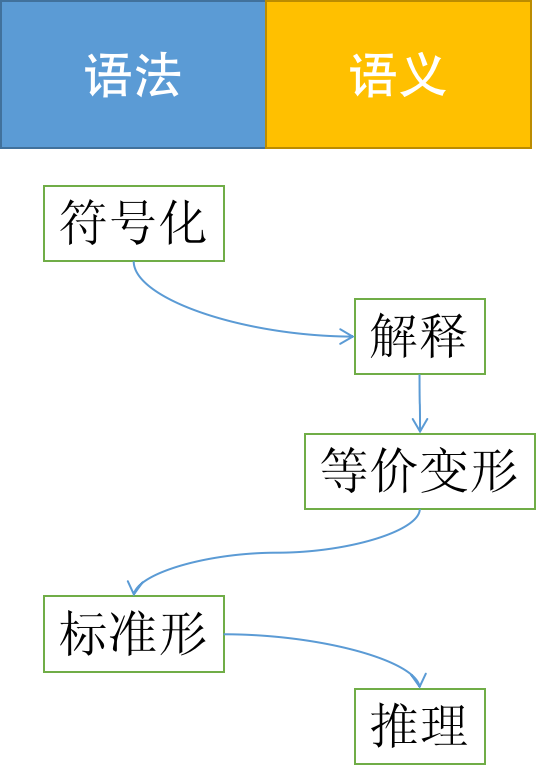
\includegraphics[scale=0.4]{2-prop-logic/figs/road-map}
	
	等价变形关注的是一个公式内部简化与变形, 推理关注的是公式与公式之间的关系. 
\end{idea}

\subsection{命题, 真值表和指派}

从高中开始, 我们似乎就开始处理各种各样的命题. 下面我们加一层抽象, 这样, 我们就可以把一些繁琐的内容交给计算机完成, 并且在探索的过程中对``什么是有效的推理''有一个更深的理解. 


\begin{definition}[命题(proposition)]
	{\bf 命题}是可以判定真假的陈述句 (不可既真又假). 其中, 称{\bf 真(true)}与{\bf 假(false)}称为命题的{\bf 真值(truth value) }. 
\end{definition}

相仿地, 我们试图像第一章探求的``最小的指令集合''一样, 问一问: 我们表达的逻辑, 有没有一些基础的组成部分? 

\begin{example}
	\begin{itemize}
		\item (高等代数) $V$可分解为$A$的特征子空间的直和, 当且仅当$A$可以对角化. 
		\item (高等数学) 如果一个数列的极限是 $A$ , 那么就是说$\forall n>N, \exists |\epsilon|\geq 0, \text{s.t.} |a_n-A|<\epsilon$.
		\item (解析几何) 两直线的方向向量$s_{1}=(l_{1},m_{1},n_{1}),s_{2}=(l_{2},m_{2},n_{2})$垂直的充要条件是$l_{1}l_{2}+m_{1}m_{2}+n_{1}n_{2}=0$;
平行的充要条件是$\frac{l_{1}}{l_{2}}=\frac{m_{1}}{m_{2}}=\frac{n_{1}}{n_{2}}.$
	\end{itemize}
\end{example}



\begin{definition}[命题逻辑的语法]
        命题逻辑的语言有且仅有如下的内容构成: 
        \begin{itemize}
            \item 任意多的命题符号
            \item 5个逻辑连接词(见表\ref{fig:conn})
            \item 左括号, 右括号
      	\end{itemize}
\end{definition}

\begin{table}
    \centering
    \begin{tabular}{|c||c|c|c|c|}
      \hline
      符号& 名称 & 英文读法 & 中文读法 & \LaTeX \\
      \hline \hline
      $\lnot$ & {negation}{(否定)} & not & 非 & \verb|\lnot| \\
      \hline
      $\land$ & {conjunction}{(合取)} & and & 与 & \verb|\land| \\
      \hline
      $\lor$ & {disjunction}{(析取)} & or & 或 & \verb|\lor| \\
      \hline
      $\to$ & conditional & {implies}{(if then)}
        & {蕴含}{(如果, 那么)} & \verb|\to| \\
      \hline
      $\leftrightarrow$ & biconditional & if and only if
        & 当且仅当 & \verb|\leftrightarrow| \\
      \hline
      \end{tabular}
    \label{fig:conn}
  \end{table}

\begin{dialogue}
	A: 为什么没有常见的``任意'', ``存在''之类的量词?
	
	B: 因为这样就复杂了. 包括结果判定的正确性和推理的难度上. 我们下一章会详细讲讲这个. 
\end{dialogue}

\begin{bonus}
	为什么叫合取, 为什么叫析取? 
\end{bonus}

其实命名的关键在于描述中的``和''和``析''. 我们可以查询古汉语字典来获取他们的意思. 并且从中找到一些合理性. 

下面, 不妨用Python语言为例, 来看一看这些内容是如何在语言中有所设计的. 需要注意的是, 上表格中的后两个记号并不是新的. 只是我们经常用他们, 于是就变成了一个独立的记号. 

如果$p$那么$q$的意思是: 如果$p$是对的, 那么$q$一定是对的, 如果$p$是错的, 那么$q$的真假性不确定. 因此, 我们可以把$p\rightarrow q$表示为$\lnot p \lor q$--意味着要么$p$不成立, 要么当$p$成立的时候$q$是对的--命题只有对和错, 所以我们就很干净的进行了一次分类讨论. 

当且仅当的表示就是``若$p$则$q$, 且若$q$则$p$''. 本质上还是命题符号之间的``非'', ``或'', ``与''之间的连接. 

\begin{example}
	命题的真假在Python中可以用布尔表达式(boolean expression)的真(true)和假(false)表示. 比如今有变量\texttt{a=True,b=False,c=True}, 那么
	\begin{lstlisting}[language=Python]
		a=True, b=False, c=True
		var = a and b or not c
		print(var)
	\end{lstlisting}
	打印的真值就是就是$a\land b\lor \lnot c$的真值. 
\end{example}

既然我们规定了符号, 自然要研究一下他们的运算律和运算关系. 什么是运算律? 

\begin{example}
	我们从小就开始听到运算律的相关内容了. 那么什么是运算律? 某国外网站的解释如下. 
	
		
The order of operations is a rule that tells the correct sequence of steps for evaluating a math expression. We can remember the order using PEMDAS: Parentheses, Exponents, Multiplication and Division (from left to right), Addition and Subtraction (from left to right).

	但是我们还听说过``交换律(commutive law)'', ``结合律(associative law)''这样的名词. 这些内容反应了我们可以如何书写, 如何计算一个表达式. 

	
\end{example}


\begin{idea}
	除了这些, 对于命题, 我们需要了解这些四个内容: 
\begin{itemize}
	\item 一个可以判定“真/假”的“东西” – 命题
	\begin{itemize}
		\item 魏恒峰是南京大学的教师.
	\end{itemize}
	\item 简单命题组成更复杂的命题 – 连接词
	\begin{itemize}
		\item 如果这门课是魏恒峰老师教的, 那么他一定是很受欢迎的. 
	\end{itemize}
	\item 深入命题的内部 – 谓词与变元
	\begin{itemize}
		\item 在“今天下雨了.”和“昨天下雨了”之间建立逻辑联系.
	\end{itemize}
	\item 体现“普遍性”与“存在性” – 量词
	\begin{itemize}
		\item 任何一个学生计算机科学的学生都值得学习魏恒峰老师的离散数学课. 
	\end{itemize}
	
\end{itemize}

现在, 我们就可以探讨更多的语义相关的内容了. 来看一看能对这个公式产生怎样的解释. 

\end{idea}

      \begin{definition}[命题符号的运算规则]
        一般地, 命题记号遵循如下的运算规则: 
        \begin{itemize}
            \setlength{\itemsep}{6pt}
            \item 最外层的括号可以省略
            \item 优先级: $\lnot$, $\land$, $\lor$, $\to$, $\leftrightarrow$
            \item 结合性: 右结合. 例如($\alpha \land \beta \land \gamma$表示$\alpha \land (\beta \land \gamma)$,
              $\alpha \to \beta \to \gamma$表示$\alpha \to (\beta \to \gamma$))
          \end{itemize}
      \end{definition}

那么我们说的命题的真假是怎么界定的呢? 通常情况下, 我们需要分类讨论每一个需要讨论的命题的真假, 最后看一看根据公式表达的真假性就行了. 所以, 我们很多时候希望``假定''这些命题的真假, 来考察最终结论的真假, 并且希望从中找到一点规律. 这样做其实有一个更专业的名字叫``真值指派''. 这样我们就可以对于``这句话永远是对的''有一个更加深刻的定义. 

\begin{dialogue}
	A: 我现在知道这些条件是, 对于明天高等数学课程的一些事情. 
	
	B: 什么事情? 
	
	A: 如果明天老师讲完了《空间立体几何》, 那么他就会做一个小测试. 同时如果我如果学的非常差的话, 并且旁边还没有大佬捞我的话, 我的平时分就非常惨淡. 
	
	B: 那我来分析一下, 假设老师没有讲完, 那么平时分暂时还不会受到影响; 如果老师讲完了, 同时我学得不差, 平时分也不会受到影响. 如果老师讲完了, 我学得非常差, 但是有人捞, 那么平时分也不会受到影响. 但是这是违反学术诚信的, 并不能做. 所以, 只要自己学得比较好才能得到很好的平时分. 
\end{dialogue}

像上面的例子, 我们通常会对命题的一些内容的真假进行预先假定, 即: 对于命题进行真值指派. 

	\begin{definition}[真值指派 ($v$)]
        令 $S$ 为一个命题符号的集合. 
        $S$ 上的一个{\bf 真值指派} $v$ 是一个从 $S$ 到真假值的映射
        \[
          v: S \to \{T, F\}.
        \]
    \end{definition}

具体的, 我们可以``指派''命题符号中的各个变量的值, 然后映射到真或假两种情况. 

我们可以借助这个想法为我们上面定义的为我们上面的逻辑连接词做一个精确的数学定义. 叫做``真值表''. 

\begin{definition}[真值表]
	表征逻辑事件输入和输出之间全部可能状态的表格. 列出命题公式真假值的表. 通常以1表示真, 0 表示假. 
\end{definition}

比如, 我们有``非''的真值表(表\ref{tab:tru-not})、``和''的真值表(表\ref{tab:tru-and})、``或''真值表(表\ref{tab:tru-or})、``若,则''真值表((表\ref{tab:tru-if-then})以及``当且仅当''的真值表(表\ref{tab:tru-iff})

\begin{table}
	\centering
	\begin{tabular}{|c|c|}
		\hline
		$p$ & $\lnot p$ \\ 
		\hline
		T & F\\ 
		F & T\\
		\hline
	\end{tabular}
	\caption{``非''的真值表}
	\label{tab:tru-not}
\end{table}

\begin{table}
	\centering
	\begin{tabular}{|c|c|c|}
		\hline
		$p$ & $q$ & $p\land q$ \\ 
		\hline
		T & T & T\\ 
		T & F & F\\
		F & T & F\\ 
		F & F & F\\
		\hline
	\end{tabular}
	\caption{``和''的真值表}
	\label{tab:tru-and}
\end{table}

\begin{table}
	\centering
	\begin{tabular}{|c|c|c|}
		\hline
		$p$ & $q$ & $p\land q$ \\ 
		\hline
		T & T & T\\ 
		T & F & T\\
		F & T & T\\ 
		F & F & F\\
		\hline
	\end{tabular}
	\caption{``或''的真值表}
	\label{tab:tru-or}
\end{table}

\begin{table}
	\centering
	\begin{tabular}{|c|c|c|}
		\hline
		$p$ & $q$ & $p\to  q$ \\ 
		\hline
		T & T & T\\ 
		T & F & F\\
		F & T & T\\ 
		F & F & T\\
		\hline
	\end{tabular}
	\caption{``如果, 那么''的真值表}
	\label{tab:tru-if-then}
\end{table}

\begin{table}
	\centering
	\begin{tabular}{|c|c|c|}
		\hline
		$p$ & $q$ & $p\land q$ \\ 
		\hline
		T & T & T\\ 
		T & F & F\\
		F & T & F\\ 
		F & F & T\\
		\hline
	\end{tabular}
	\caption{``当且仅当''的真值表}
	\label{tab:tru-iff}
\end{table}

\begin{prob}
	人类学者埃贝尔考察一个有着许多古怪社会现象的群岛,他到访的第一个小岛上的居民分为两类,而且每人必属其中的一类:
	\begin{itemize}
		\item Knight: 这类人永远说真话
		\item Knave: 这类人永远说假话
	\end{itemize}
	在岛上埃贝尔遇到一行三人,且称他们为 A, B, C。
埃贝尔问A: “你是knight还是knave?” A回答了,但埃贝尔没听清;
于是埃贝尔就问B: “他(A)说的是什么?” B告诉埃贝尔A说自己是knave。

此时,C插话说:“别相信他(B),他说谎!”

我们的问题是:C是 knight 还是 knave?
\end{prob}

事实上, 我们在小学很可能通过列举的方法完成求解. 但是现在我们可以用真值表列举. 甚至可以把公式写出来进行推演! 

\begin{bonus}
	等等, 什么叫推演? 有哪些推演规律? 这些推演规律是不是可以用公式表示? 这些都是下一节要介绍的内容. 
\end{bonus}

比如一个命题的否定的否定还是原命题本身一样, 我们可以定义一些``公式''. 比如$\not \not p$与$p$等价. 首先我们定义一下什么叫``满足'', ``蕴含''或者``等价''. 

\begin{definition}[满足 (Satisfy)]
        如果 $\overline{v}(\alpha) = T$, 则称真值指派 $v$ {\bf 满足}公式 $\alpha$. 
      \end{definition}

      很多时候一些逻辑表达式看上去就是废话. 比如``如果我后天知道了考试的成绩, 那我明天就知道了''. 数学上面对这类问题有一个定义叫做``重言蕴含''. 

      \begin{definition}[重言蕴含 (Tautologically Implies)]
          设 $\Sigma$ 为一个公式集. 
    
          $\Sigma$ {\bf 重言蕴含}公式 $\alpha$,
          记为 $\Sigma \models \alpha$,
    
          如果{每个}满足 $\Sigma$ 中{所有}公式的真值指派都满足 $\alpha$. 
      \end{definition}

      \begin{definition}[重言式/永真式 (Tautology)]
        如果将等价词两侧的子公式各自看作表达式,则这两个逻辑表达式对于相关逻辑变量的任意赋值有相同的逻辑值. 
        (或者: 如果 $\emptyset \models \alpha$, 则称 $\alpha$ 为{\bf 重言式},
        记为 $\models \alpha$.)
      \end{definition}

      反之, 就是永远都不能成立的矛盾的形式. 
      
      \begin{definition}[矛盾式/永假式 (Contradiction)]
        若公式 $\alpha$ 在所有真值指派下均为假, 则称 $\alpha$ 为{\bf 矛盾式}. 
      \end{definition}

      \begin{definition}[重言等价 (Tautologically Equivalent)]
        如果 $\alpha \models \beta$ 且 $\beta \models \alpha$,
        则称 $\alpha$ 与 $\beta$ {\bf 重言等价}, 记为 $\alpha \equiv \beta$. 
      \end{definition}
      
     对于命题公式而言, 如果对于相同的变量输入, 外部观测的结果的真假相同, 我们就称为命题的等价. 
     
     \begin{definition}[命题的等价]
     	设$G,H$是两个命题公式, $P_1,\cdots, P_n$是出现在命题$G,H$中的所有变元, 如果对于$P_1,P_2,\cdots,P_n$的$2^n$组不同的解释, $G,H$的真值结果都相同, 那么称$G$和$H$是等价的, 记作$G\Leftrightarrow H$. 
     \end{definition}      
     根据上面的定义, 我们可以证明: 
     \begin{theorem}
     	$G\Leftrightarrow H$的充分必要条件是$G\leftrightarrow H$. 
     \end{theorem}
     
     \begin{bonus}
     	永真式和等价有什么区别和联系? 
     	
     	A proposition that is always True is called a tautology. Two propositions $p$ and $q$ are logically equivalent if their truth tables are the same. Namely, $p$ and $q$ are logically equivalent if $p \leftrightarrow q$ is a tautology. If $p$ and $q$ are logically equivalent, we write $p \Leftrightarrow q$.
     \end{bonus}
      
\subsection{命题逻辑的化简}

在上面我们发现了有很多的``废话'', 但是, 当看上去是``废话''的东西堆多堆复杂的时候, 那么它就不是显然的. 这就需要一些推理规律来帮助我们联通看上去毫不相干的逻辑符号. 

经过我们的探讨, 我们就希望把一些最基本的规律写出来: 

\begin{proposition}(一些永真的公式)
如果$A,B,C$是命题, 那么以下的内容是永真式: 
        \begin{itemize}
            
            \item 交换律:
          \[
            (A \land B) \leftrightarrow (B \land A)
          \]
          \[
            (A \lor B) \leftrightarrow (B \lor A)
          \]
        \item 结合律:
          \[
            ((A \land B) \land C) \leftrightarrow (A \land (B \land C))
          \]
          \[
            ((A \lor B) \lor C) \leftrightarrow (A \lor (B \lor C))
          \]
        \item 分配律:
          \[
            (A \land (B \lor C)) \leftrightarrow ((A \land B) \lor (A \land C))
          \]
          \[
            (A \lor (B \land C)) \leftrightarrow ((A \lor B) \land (A \lor C))
          \]
        \item De Morgan律: 
          \[
            \lnot (A \land B) \leftrightarrow (\lnot A \lor \lnot B)
          \]
          \[
            \lnot (A \lor B) \leftrightarrow (\lnot A \land \lnot B)
          \]
          \item 双重否定律:
            \[
                \lnot \lnot A \leftrightarrow A
            \]
            \item 排中律:
            \[
                A \lor (\lnot A)
            \]
            \item 矛盾律:
            \[
                \lnot (A \land \lnot A)
            \]
            \item 逆否命题:
            \[
                (A \to B) \leftrightarrow (\lnot B \to \lnot A)
            \]
        \end{itemize}
        
      \end{proposition}

利用这些内容我们可以构造一些等价的命题: 

\begin{proposition}[基本等价定律]
	(1) 幂等律: $E_1:G\land G\Leftrightarrow G; E_2:G\lor G\Leftrightarrow G;$
	
	(2) 交换律: $E_3: G\an H \eqw H \an G; E_4: G\oi H \eqv H \oi G;$
	
	(3) 结合律: $E_5: G\an(H\an S)\eqw (G\an H)\an S; E_6: G\oi(H\oi S)\eqw (G\oi H)\oi S$
	
	(4) 分配律: $E_7: G\oi(H\an S) \eqw (G\oi H)\an (G\oi S); E_8: G\an (H\oi S)\eqw (G\an H)\oi (G\oi S)$
	
	(5) 吸收律: $E_9: G\oi (G\an H)\eqw G; E_{10}: G\an (G\oi H)\eqw G$
	
	(6) 同一律: $E_{11}: G\oi \texttt{False}\eqw G; E_{12}: G\an \texttt{true}\eqw G$
	
	(7) 零律: $E_{13}: G\oi \texttt{True}\eqw \texttt{True}; E_{14}: G\an \texttt{False}=\texttt{False}$
	
	(8) 双重否定律: $E_{15}: \no (\no G)\eqw G$
	
	(9) De Morgan律: $E_{16}: \no (G\oi H)\eqw \no G \an \no H; E_{17}: \no (G\an H)=\no G\oi \no H$
	
	(10) 矛盾律: $E_{18}:G\an \no G\eqw \texttt{False}$
	
	(11) 排中律: $E_{19}:G\oi \no G\eqw 1$
	
	(12) 等价式: $E_{20}:G\leftrightarrow \eqw (G\to H)\an (H\to G)$
	
	(13) 蕴含式: $E_{21}: G\to H\eqw \no G\oi H$
	
	(14) 假言易位: $E_{22}: G\to H \eqw \no H\to \no G$
	
	(15) 等价否定形式: $E_{23}: G\lrarr H \eqw \no G\lrarr \no H$
	
	(16) 归谬论: $E_{24}: (G\to H)\an (G\to \no H) \eqw \no G$
	
	% TODO: On Sun Feb 26, wrote here
\end{proposition}

这些为什么有用呢? 考虑有一天你在求解一个数学问题, 其中你想把一个命题否定掉, 比如

\begin{prob}
	如果$P,Q,R$是命题, 请否定$P\to Q\land R$. 
\end{prob}

其中一个很重要的手段就是通过上面的这些重言式的替换. 就像在学习三角函数的时候使用三角恒等式替换一样. 

下面我们来看一个比较有趣的逻辑代数推演的例子: 
\begin{prob}
	我们已经知道 Bill, Jim和Sam分别来自Boston, Chicago和 Detroit. 以下每句话半句对,半句错:
	\begin{itemize}
		\item Bill来自Boston($p_1$), Jim来自Chicago($p_2$).
		\item Sam来自Boston($p_3$), Bill来自Chicago($p_4$).
		\item Jim来自Boston($p_5$), Bill来自Detroit($p_6$).
	\end{itemize}
	能确定每个人究竟谁来自何处吗?
\end{prob}

\begin{sol}
	我们可以将上述条件用以下逻辑表达式来表示:
$$
\red{((p_1\land \lnot p_2)\lor (\lnot p_1\land  p_2))\land ((p_3\land \lnot p_4)\lor (\lnot p_3\land  p_4))}\land ((p_5\land \lnot p_6)\lor (\lnot p_5\land  p_6))
$$

先看前两个括号(上述式子红色的部分), 以连接两个式子中间的$\land$展开(下式红色符号), 我们有
$$
\begin{aligned}
	&((p_1\land \lnot p_2)\teal{\lor} (\lnot p_1\land  p_2))\red{\land} ((p_3\land \lnot p_4)\teal{\lor} (\lnot p_3 \land  p_4)) \\
	=& (p_1\land \lnot p_2 \red{\land} p_3\land \lnot p_4) \teal{\lor} (p_1\land \lnot p_2 \red{\land} \lnot p_3\land  p_4)\teal{\lor} (\lnot p_1\land  p_2)\red{\land}\lnot p_3\land  p_4)\teal{\lor} (\lnot p_1\land  p_2\red{\land}\lnot p_3\land  p_4)
\end{aligned}
$$
根据已知条件, $p_1\land p_4, p_2\land p_4, p_1 \land p_3$均为假的, 所以上述式子是
$$
(\lnot p_1 \land p_2 \land p_3 \land \lnot p_4)
$$

与后面的$((p_5\land \lnot p_6)\lor (\lnot p_5\land  p_6))$进行$\land$操作, 也就是有

$$
\begin{aligned}
	&(\lnot p_1 \land p_2 \land p_3 \land \lnot p_4)((p_5\land \lnot p_6)\lor (\lnot p_5\land  p_6)) \\
	=& (\lnot p_1 \land p_2 \land \red{p_3} \land \lnot p_4 \land\red{ p_5} \land \not p_6)\lor (\lnot p_1 \land p_2 \land p_3 \land \lnot p_4 \land \lnot  p_5 \land p_6) \\
	=&(\lnot p_1 \land p_2 \land p_3 \land \lnot p_4 \land \lnot  p_5 \land p_6)
\end{aligned}
$$

所以我们知道: $p_2, p_3, p_6$是对的. 
\end{sol}

事实上, 我们能这样做是因为有带入定理帮助我们. 

\begin{theorem}[带入定理]
	运用永真式代替命题的变元, 得到的命题结果与原命题等价. 
\end{theorem}

\begin{bonus}
	缺失的证明: 为什么没有了定理的证明? 	
	
	一个很重要的问题是我们数学的基石是缺失的. 其实, 人类在认识世界的时候开始也是缺乏基础的, 仅仅凭借直觉来建立一些体系. 直到直觉无法完全覆盖的时候, 人类才开始探索有没有什么基础的支撑点来支持这一系列理论. 
\end{bonus}

\subsection{化简的目标: 范式}

范式的意思是``规范的形式''. 那么, 这些内容化简到最后有没有一个目标呢? 其实是有的. 任何一个命题都可以写成``合取范式(CNF)''或者``析取范式(DNF)''的形式. 下面给出形如这样的式子的定义:

 
\begin{definition}[合取范式 (Conjunctive Normal Form)]
            我们称公式 $\alpha$ 是{\bf 合取范式}, 如果它形如
            \[
              \alpha = \beta_{1} \land \beta_{2} \land \dots \land \beta_{k},
            \]
            其中, 每个 $\beta_{i}$ 都形如
            \[
              \beta_{i} = \beta_{i1} \lor \beta_{i2} \lor \dots \lor \beta_{in},
            \]
            并且 $\beta_{ij}$ 或是一个命题符号, 或者命题符号的否定. 
    \end{definition}


   \begin{definition}[析取范式 (Disjunctive Normal Form)]
            我们称公式 $\alpha$ 是{\bf 析取范式}, 如果它形如
            \[
              \alpha = \beta_{1} \lor \beta_{2} \lor \dots \lor \beta_{k},
            \]
            其中, 每个 $\beta_{i}$ 都形如
            \[
              \beta_{i} = \beta_{i1} \land \beta_{i2} \land \dots \land \beta_{in},
            \]
            并且 $\beta_{ij}$ 或是一个命题符号, 或者命题符号的否定. 
    \end{definition}

\begin{theorem}
	每一个命题都有等价的合取范式和析取范式的形式. (Given any proposition, there exists a proposition in disjunctive normal form which is equivalent to that proposition.)
\end{theorem}

\begin{dialogue}
A: 你真的想要看证明吗?

B: 嗯... 有点好奇. 

A: 好, 给你看看. 不过有一些集合论的内容, 我们会在后面会讲解. 

\end{dialogue}


\begin{proof}
	(Copied from \url{https://planetmath.org/everypropositionisequivalenttoapropositionindnf} ) Any two propositions are equivalent if and only if they determine the same truth function. Therefore, if one can exhibit a mapping which assigns to a given truth function 
 a proposition in disjunctive normal form such that the truth function $f$ of this proposition is $f$, the theorem follows immediately.

Let $n$ denote the number of arguments $f$ takes. Define
$$
V(f)=\set{X\in\set{T,F}^n,f(X)=T}
$$
For every $X\in \set{T,F}$, define $L_i (x) = \set{T,F}^n \to \set{T,F}$ as follows: 
$$
L_i (X)(Y)=  \begin{cases}
	Y_i , X_i =T;\\
	\lnot Y_i , X_i =F.
\end{cases}
$$
Then, we claim that 
$$
f(Y)=\bigwedge_{x\in V(f)}\bigvee_{i=1}^nL_i(X)(Y)
$$
On the one hand, suppose that $f(Y)=T$ for a certain $Y\in \set{T,F}^n$, By definition of $V(f)$, we have $Y\in V(f)$. By definition of $L_i$, we have
$$
L_i (Y)(Y)=\begin{cases}
	Y_i , Y_i =T\\
	\lnot Y_i, y_i = F 
\end{cases}
$$
In either case, $L_i(Y)(Y)=T$, since a conjunction equals $T$ if each term of the conjunction equals $T$, it follows that$\bigvee_{i=1}^nL_i(Y)(Y)=T$, Finally, since a disjunction equals $T$ if and only if there exists a term which equals $T$, it follows the right hand side equals equals $T$ when the left-hand side equals $T$.

On the one hand, suppose that $V(Y)+F$ for a certain $Y\in\set{T,F}$. Let $X$ be any element of $V(f)$. Since $Y \notin V(f)$, there must exist an index $i$ such that $X_i\neq Y_i$. For this choice of $i$, $Y_i =\lnot X_i $, Then we have
$$
L_i (X)(Y)=\begin{cases}
	\lnot X_i , X_i=T\\
	\lnot \lnot X_i, X_i =F
\end{cases}
$$
In either case,$L_i(X)(Y)=F$, Since a conjunction equals $F$ if and only if there exists a term which evaluates to $F$, it follows that $\bigvee_{i=1} ^n=F$ for all $X\in V(f)$. Since a disjunction equals 
 if and only if each term of the conjunction equals $F$, it follows that the right hand side equals equals $F$when the left-hand side equals $F$.

\end{proof}

\begin{dialogue}

B: 看不懂的证明还有意义吗?

A: 这是一个很好的问题. 看似看不懂, 但是你在阅读的过程中会无意间记住一些话语, 那么将来你碰见相似的东西的时候, 就会感到快乐, 大多数情况下就更容易理解了. 

B: 感觉我没办法一步到位诶...

A: 是的, 我们认识世界也是这样的, 一步一步的向前推进. 我们可以先有一个直观的印象, 慢慢做更加详细的探讨. 		
\end{dialogue}


上面的只是给了我们一个正确性证明, 但是并没有告诉我们如何把一个式子化为合取范式或者析取范式. 一般的, 我们有如下的方法: 

(1)用$\lnot,\land,\lor$代替$\to,\leftrightarrow$;

(2)用双重否定律, 消去律去掉多余的否定连接词, 运用De Morgan律将否定连接词内移. 

(3) 利用分配率, 结合律, 幂等律整理得到. 

实际上, 在上面的三个人从哪里来的例子中, 我们就用到了这样的想法. 


\begin{bonus}
	为什么合取范式(外面$\land$里面$\lor$)和析取范式(外面$\lor$里面$\land$)这么重要? 
\end{bonus}

下面的这个回答来源于StackExchange上面的回答\cite{why-important-cnf-dnf}, 简要概括如下:

逻辑公式中的变量(输入)可以以复杂的方式混在一起. 如果公式采用CNF或DNF,变量就更加分离,从而更容易看出表达式何时成立. 比如, 要检查CNF是否成立,只需逐个检查每个子句有一个是假的整个都是假的. DNF也类似: 逐个检查子句,并在找到一个为真的子句时停止, 整个句子都是真的. 

很多时候真值表会带来很多的麻烦: 意味着穷举和非常麻烦的事情. 有了CNF与DNF以后, 我们不必从真值表开始枚举, 可以通过操作表达式来形式地构造标准形式. 在某些情况下可能可以更方便一些.

下面我们来看一看合取范式与析取范式的一些性质. 

我们发现, 在合取范式中, 只要有一个条件是假的, 那么整个命题都是假的. 在析取范式中, 只要有一个条件是真的, 那么这个命题是真的. 特别地, 如果每个命题变元或其否定恰好只有一个出现过并且只出现了一次, 那么我们说这个合取范式为极小项(析取范式为极大项). 比如我们有两个变量, 那么就可以有如下的四个逻辑表达式: 
$$
P\land Q \qquad
 \lnot P \land Q \qquad
  P \land \lnot Q \qquad
   \lnot P \land \lnot Q \qquad
$$

这样就保证了我们除了枚举输入的命题之外, 我们还可以枚举极小项, 极大项, 从两方面来观察命题的真假. 比如. 还是上面的两个命题符号的情形, 对于合取范式和析取范式, 分别有表\ref{tab:min} 以及表\ref{tab:max}的情形. 

\begin{table}
	\centering
	\begin{tabular}{|c|c|c|c|c|}
		\hline
		P Q & $\lnot P \land \lnot Q$ & $\lnot P \land  Q$ & $P \land \lnot Q $& $ P \land  Q$\\
		\hline
		0 0 & 1 & 0 & 0 & 0\\
		0 1 & 0 & 1 & 0 & 0\\
		1 0 & 0 & 0 & 1 & 0\\
		1 1 & 0 & 0 & 0 & 1\\
		\hline
	\end{tabular}
	\label{tab:min}
	\caption{合取范式枚举命题符号是否取反以及指派为真假的情形(极小项)}
\end{table}

\begin{table}
	\centering
	\begin{tabular}{|c|c|c|c|c|}
		\hline
		P Q & $\lnot P \land \lnot Q$ & $\lnot P \land  Q$ & $P \land \lnot Q $& $ P \land  Q$\\
		\hline
		0 0 & 0 & 1 & 1 & 1\\
		0 1 & 1 & 0 & 1 & 1\\
		1 0 & 1 & 1 & 0 & 1\\
		1 1 & 1 & 1 & 1 & 0\\
		\hline
	\end{tabular}
	\label{tab:max}
	\caption{合取范式枚举命题符号是否取反以及指派为真假的情形(极大项)}
\end{table}

\begin{bonus}
	列表有什么好处? 我们可以发现什么规律? 
\end{bonus}

我们发现每一个赋值对应一个取值为$\frac{\text{真}}{\text{假}}$的极$\frac{\text{小}}{\text{大}}$项, 每个极$\frac{\text{小}}{\text{大}}$项的$\frac{\text{真}}{\text{假}}$赋值是唯一的. 并且没有等价的两个极$\frac{\text{小}}{\text{大}}$项, 任何两个不同的极$\frac{\text{小}}{\text{大}}$项$\frac{\text{合}}{\text{析}}$取必为真, 极$\frac{\text{小}}{\text{大}}$的否定是极$\frac{\text{大}}{\text{小}}$, 所有的极$\frac{\text{小}}{\text{大}}$项的$\frac{\text{析}}{\text{合}}$取为永假公式. 

\begin{dialogue}
	A: 这个和二进制表示好像. 我们能不能有一种方法来用一个整数来表示命题? 
	
	B: 确实, 但是需要考虑一下命题变元的记号问题. 
\end{dialogue}

如果我们把合取范式和析取范式里面的内容都变为极小项/极大项的时候, 我们就可以得到更标准, 更易于处理的内容. 通常称为\textbf{主合(析)取范式}. 

\section{命题推演的真象: 命题的推演}

我们发现, 蕴含词的逻辑永真式和我们经常所做的推理有很好的联系. 具体地, 如果$\alpha \to \beta$, 那么如果$\alpha$成立, 可以\textbf{推导}出$\beta$为真. 

同样的, 如果假设$\alpha$成立, 只要经过合理的推导可以\textbf{推导}出$\beta$为真, 那么这个规则就是成立的.  


我们在推理时多半用“因为...所以...”, 那么前面的什么概念能起关键作用呢?

一般而言, 逻辑推理有一系列的假设前提$A_1,A_2,\cdots,A_n$, 有一个结论$B$, 什么是正确的推理呢? 形式化地, 对前提与结论所涉及的逻辑变量任意赋值, 如果任意的$A_i$均为这真, 它们的合取式的值当然也为真, 那么$B$必为真. 

形式化的, 我们就说: 这样的推理是正确的. 

\begin{definition}
	设$G_1,G_2,\cdots,G_n,H$是命题公式, 对任意指派$I$, 如果$G_1\land G_2\land \cdots\land G_n$为真, $H$也为真, 或者$G_1\land G_2\land \cdots\land G_n$为真, $H$为假, 那么称$H$是$G_1, G_2, \cdots, G_n$的逻辑结果. 或者$G_1, G_2, \cdots, G_n$共同蕴含$H$, 记做$G_1\land G_2\land \cdots\land G_n\Rightarrow H$. 
\end{definition}


\begin{theorem}
	公式$H$是前提集合$\set{G_1,G_2,\cdots,G_n}$的逻辑结果当且仅当$G_1\land G_2\land \cdots\land G_n\to H$为永真的公式. 
\end{theorem}

需要注意的是, $\Rightarrow$是一个关系, 这是一个不可计算的公式. 

\begin{definition}
	设$G_1, G_2, \cdots, G_n,H$是命题公式, 如果$H$是$G_1, G_2, \cdots, G_n$的逻辑结果, 那么称$G_1, G_2, \cdots, G_n\Rightarrow H$是有效的或正确的. 否则称为无效的. 
	
	称$G_1, G_2, \cdots, G_n$为一组前提, $H$为结论, 如果记$\Gamma=\set{G_1,G_2,\cdots,G_3}$, 上述关系可以记作$\Gamma\Rightarrow H$. 
\end{definition}

\begin{dialogue}
	A: 如果我有一个有效的推理, 那么结论应该是正确的吧? 
	
	B: 那可不一定. 举个例子: $1+1=3, 2+2=4 \Rightarrow 114+514=191$虽然形式是有效的, 但是结论确实是不对的.
	
	A: 确实, 很像是$\rightarrow$记号的拓展. 如果前提条件为假, 那么就不关心结论的正确性了. 
\end{dialogue}

所以这就解释了我们为什么经常使用的因为...所以...是合理的了. 比如$(p\land(p\land q))\to q$是永真的, 那么就可以有三段论这样的合理的推理过程了. 

\begin{example}
	一个三段论的示例如下: 
	
	关爱学生, 好好讲课, 有真才实学的老师会被学生欢迎
	
	朱富海老师关爱学生, 好好讲课, 有真才实学
	
	朱富海老师受学生欢迎. 
\end{example}

我们经常对于知识研究一些规律. 比如在逻辑公式很长的时候, 逐个枚举是十分低效率的. 比如, 如果有200个命题符号的逻辑公式, 用计算机枚举则需要$2^{200}$种情况. 用Python的强大的计算器可以知道, 需要核验的情况是一个61位数.

\begin{example}
	我们可以使用\texttt{ipython}中输入\texttt{len(str(2**200))}知道它的位数. Python自带高精度计算, 因此如果直接输入\texttt{2**200}, 它就会直接把数字算出来! 
\end{example} 

既然要推理, 我们就要有推理的\textbf{定律}和推理的推理的\textbf{规则}. 正如前面说的程序语言的语法和语义类似. 

经过总结归纳, 我们有如下的推理定律: 

\begin{theorem}[常见的推理定律]
	设$G,H,I,J$是任意的命题公式, 那么我们有: 
	
	(1) 简化规则: $I_1:G\land H\Rightarrow G$, $I_2: G\land H \Rightarrow H$.
	
	(2) 添加规则: $I_3:G\Rightarrow G\lor H$, $I_4: H\Rightarrow G\land H$.
	
	(3) $I_5: G,H\Rightarrow G\land H$.
	
	(4) 选言三段论: $I_6: \lnot G, G\lor H \Rightarrow H$.
	
	(5) 分离规则: $I_7: G,G\to H\Rightarrow H$.
	
	(6) 否定结论: $I_8: \lnot H, G\to H\Rightarrow \lnot G$.
	
	(7) 连续推理: $I_9: G\to H, H\to I\Rightarrow G\to I$.
	
	(8) 两难推理: $I_10: G\lor H,G\to I, H\to I\Rightarrow I$

\end{theorem}

一个学习的很好的方法是举一些例子. 我们可以用上面的符号翻译成具体的例子. 不用太过于拘束.  

\begin{idea}
	遇见新概念的时候, 可以应该举一些例子辅助理解, 尽可能弄懂来龙去脉. 
\end{idea}

以最后一个例子为例, 有: 

\begin{example}
	\begin{itemize}
		\item[8] 现在发动机坏了并且没油了. 如果发动机坏了, 车子就动不了了; 如果没油了, 车子就动不了了; 我们可以得到: 车子动不了了. 
	\end{itemize}
\end{example}

\begin{bonus}
	为什么叫他们为基础的规则? 是不是因为他们具有某种完备性? 
\end{bonus}


推理规则可以使用真值表验证. 除此之外, 我们还需要推理定律: 也就是需要完成什么样的变换. 我们有三条规则.


(1) Premise规则: 前提引用. 如果推理的时候引入了前提集合中的一个前提, 那么称为使用了P规则;

(2) Transformation规则: 逻辑结果引用的规则. 在推理过程中, 如果引入推理过程中某个产生的中间结果, 那么称使用了T规则;

(3) Conclusion premise规则: 附加前提规则. 在推理过程中, 如果逻辑结果为一个含有蕴含$\rightarrow$的式子, 那么把它的前提条件作为假设引入, 就是用了$CP$规则. 所有引入的假设最终必须被``{\bf 释放}'' (discharged)
    所谓释放, 其实就是在使用假设$\alpha$作为假设的前提下推出了$\beta$, 最后要写成$\alpha \rightarrow \beta$的形式. 这就是假设的释放. 

我们来推导一下$I_6$. 

\begin{proof}
	(1) 直接引入前提集合的前提, 有$\lnot G$;
	
	(2) 直接引入前提集合的前提, 有$G \land H$;
	
	(3) 使用(1),(2)的中间结果, 有$\lnot G \land (G\lor H)$;
	
	(4) 使用(3)的中间结果, 使用分配律,有$(\lnot G \land G)\lor (\lnot G \land H)$;
	
	(5) 使用(4) 的中间结果, 有$\lnot G \land H$;
	
	(6) 使用(5)的中间结果, 有$H$. 
\end{proof}

对于$I_9$, 我们可以先把$G$是对的引入集合, 然后最后推理得到$I$的时候, 为了说明它的正确性, 就需要使用CP规则. 

\begin{bonus}
	P规则和T规则能足够做所有的内容的推理吗?
\end{bonus}

在上面我们做的研究中, 我们会发现很多东西相当的机械化. 于是, 在有机械化的内容出现的时候, 计算机就有用了. 所以, 我们希望找到一种方法, 使得计算机可以自动地推理我们的命题. 在1965年, J.A. Robinson发现了消解原理: 它的原理是规则$I_7$. 具体的有: 

\begin{definition}[消解与消解式]
	设$G$和$H$是两个析取式, 如果$G$中有变元$P,H$中有变元$\lnot P$, 则从$G$和$H$中分别消去$P$和$\lnot P$, 并且将余下的部分析取, 构成新的表达式$W$, 这个过程称为消解. $W$为$G,H$的消解式. 
\end{definition}

我们经过消解的方法, 立即可以得到一个很有``自动化''意思的定理: 

\begin{theorem}
	如果$W$是$G,H$的消解式, 则$G\land H\Rightarrow W$. 
\end{theorem}

\section{表达更丰富的内容: 谓词~部分与整体的关系}

我们发现命题逻辑无法表达部分与整体的关系. 例如: 

\begin{example}
	(1) 张三是个法外狂徒; 
	
	(2) 李四与张三是好朋友;
	
	(3) 李四也是一个法外狂徒;
	
	(4) 王五站在张三与李四中间;\footnote{王五害怕极了...} 
	
	(5) 王五长得比张三与李四都高;
	
	(6) 所有的法外狂徒终将绳之以法;
	
	(7) 存在法外狂徒改过自新. 
\end{example}


我们发现以前学过的东西仅仅能应对很基本的内容. 比如任意, 存在无法表示. 下面我们形式化的先来说说什么是任意和存在. 这些是对于一类类似于变元的内容的性质的总体描述. 因此,  我们首先定义什么是谓词

\begin{definition}[谓词(predicate)]
	在不能被拆分为更小的命题中(通常叫做原子命题(automic expression)), 可以独立存在的客体(subject)(通常是句子中的主语, 宾语)称为个体词(individual), 描述客体的性质或客体之间的关系的部分称为谓词. 
\end{definition}

很多时候, 我们会泛指一些很笼统的概念, 比如``人''. 也有时候我们会举一些明确的个体, 比如``蒋炎岩老师''. 这时候我们就需要区分``个体变量''(通常是泛指)和``个体常量''(通常是特指).

\begin{definition}[个体常量, 个体变量, 个体域, 全总个体域]
	对于具体明确的个体而言, 称为个体常量(individual constant), 一般用形如$a,b,a_1,b_1$这样的小写字母表示. 个体变量(individual variable)取值范围称作个体域(或论域, individual field), 通常用字母$D$表示. 我们通常把宇宙间所有个体聚集在一起的个体域称为全总论域(universual individual field). 
\end{definition}  

\begin{definition}[$n$元命题函数]
	设$P(x_1,x_2,\cdots,x_n)$是$n$元函数(function), 其中每一个变量可以取其可以取到的对应的值. 如果$P$的值域是$\set{0,1}$, 那么说$P(x_1 ,x_2, \cdots, x_n)$是$n$元命题函数或$n$元谓词(n-ary propositional function).  
\end{definition}

这样子, 我们就可以更加方便的定义量词(qualifier)了. 

\begin{definition}[全称量词与特称量词]
	表达全部数量关系的词语诸如``一切'',``所有'',``每一个''等称为全称量词(universal quantifier), 记作$\forall$. 如所有的$x$记作$\forall x$. 
	
	表达部分数量关系的词语诸如``存在'', ``有一个'', ``有一些''称为存在量词(existential quantifier). 记作$\exists$. 如有一些$x$记作$\exists x$. 
	
	这里面, $x$被称为作用变量(function variable), 一般将量词加在对应的谓词之前, 如$\forall x. F(x)$或$\exists x. F(x)$. 此时$F(x)$被称为全称量词和存在量词的作用域(又成为辖域, scope). 
\end{definition}

上面的内容一个很重要的地方在于引入了变元. 例如, 在函数符号和谓词符号中, 变元的引入使得我们要讨论的事情变得更加多了. 

\begin{bonus}
	你在哪里还见到过由常数引入到变量? 其实, 我们在初中的时候, 先研究了二次方程的解, 再把$x$当做一个变元, 研究所有$x$构成的二元组$(x,f(x))$的一些性质. 有兴趣学习高等代数的同学会发现在引入$\lambda-\text{矩阵}$的时候也用了这样的知识. 
\end{bonus}

这下子, 我们就可以定义谓词逻辑的构成了. 

\begin{definition}[谓词逻辑的构成] 谓词逻辑由且仅有以下的几部分构成: 

      (1)逻辑联词: $\lnot, \land, \lor, \to, \leftrightarrow$
      
      (2)量词符号:  $\forall$ (forall; 全称量词),
        $\exists$ exists; 存在量词)
      
      (3)变元符号: $x, y, z, \dots$
      
      (4)左右括号: $(, )$
      
      (5)常数符号: 零个或多个常数符号 $a, b, c, \dots$, 表达特殊的个体
      
      (6)函数符号: $n$-元函数符号 $f, g, h, \dots$ ($n \in \N^{+}$), 表达个体上的运算
      
      (7)谓词符号:  $n$-元谓词符号 $P, Q, R, \dots$ ($n \in \N$), 表达个体的性质与关系
    
\end{definition}





和普通公式一样, 谓词公式也是由一项一项构成的.

\begin{definition}[项 (Term)]
  \begin{enumerate}
    \item 每个变元 $x, y, z, \dots$ 都是一个项;
    \item 每个常数符号都是一个项;
    \item 如果 $t_{1}, t_{2}, \dots, t_{n}$ 是项,
      且 $f$ 为一个 $n$-元函数符号, \\
      则 $f(t_{1}, t_{2}, \dots, t_{n})$ 也是项;
    \item 除此之外, 别无其它. 
  \end{enumerate}
\end{definition}

\begin{definition}[公式 (Formula)] 谓词逻辑的公式定义如下: 
  \begin{itemize}
    \item 如果 $t_{1}, \dots, t_{n}$ 是项, 且 $P$ 是一个 $n$ 元谓词符号, \\
      则 $P(t_{1}, \dots, t_{n})$ 为公式, 称为{\bf 原子公式};
    \item 如果 $\alpha$ 与 $\beta$ 都是公式, 则 $(\lnot \alpha)$
      与 $(\alpha \;\red{\ast}\; \beta)$ 都是公式;
    \item 如果 $\alpha$ 是公式, 则 \red{$\forall x.\; \alpha$}
      与 \red{$\exists x.\; \alpha$} 也是公式;
    \item 除此之外, 别无其它. 
  \end{itemize}
\end{definition}

我们来举一些例子: 

\begin{example}
	\begin{itemize}
    \item 0 不是任何自然数的后继
        \[
          \forall x.\; \lnot (Sx = 0)
        \]
      \item 两个自然数相等当且仅当它们的后继相等
        \[
          \forall x.\; \forall y.\; (x = y \leftrightarrow Sx = Sy)
        \]
      \item $x$ 是素数 ($x > 1$ 且 $x$ 没有除自身和1之外的因子)
        \[
          \text{Prime}(x): S0 < x \land \forall y.\; \forall z.\; (y < x \land z < x) \to \lnot (y \times z = x)
        \]
      \item 哥德巴赫猜想 (任一大于2的偶数, 都可表示成两个素数之和)
        \begin{align*}
          &\forall x.\; (SS0 < 2 \land (\exists y.\; 2 \times y = x)) \to \\
            &\quad (\exists x_{1}.\; \exists x_{2}.\; \text{Prime}(x_{1}) \land \text{Prime}(x_{2})
              \land x_{1} + x_{2} = x)
        \end{align*}
  \end{itemize}

\end{example}

\begin{quote}
有了坐标系, 辩证法进入了数学. 有了坐标系, 运动进入了数学. \\
\hfill --Engels
\end{quote}

这里的``运动'', ``坐标系''只是变量引入数学的结果. 自然, 这让我们探索的内容更加的丰富, 同时也更加容易犯错了. 比如, 我们很多时候喜欢对变量做替换. 但是, 下面的代换显然是错的: 

\begin{example}
	``那曲市'' := ``中国最大的城市''
	
	``那曲市''有三个汉字
	
	``中国最大的城市''有三个汉字
\end{example}

因为``中国最大的城市''这个字符串有7个汉字构成. 这就警告我们要在变量代换的时候要格外小心. 那么, 变量有哪些类型呢? 

在公式$\forall x. P(x,y)\lor \exists y. R(x,y)$中, 根据量词作用域的定义, $\forall x$的作用域是$P(x,y)$, 因此$x$受到了$\forall x$的约束, 从而把这个变元称作{\bf 约束变元}. 然而这个的$y$没有受到$\forall x$的约束, 所以称为{\bf 自由变元}. 

\begin{definition}[约束变元与自由变元]
	给定公式$\forall x. G$和$\exists x.G$, $G$为$\forall x$和$\exists x$的作用域, 那么$G$中的$x$出现的都是约束出现(bounded occurrence), 称变元$x$则是约束变元(bound variable), $G$中不同于$x$的其他变元出现的则是自由出现(free occurrence), 称这些变元为自由变元(free variable)
\end{definition}

\begin{dialogue}
	A: 这就像C语言里面判断一个变量是不是被定义过了一样! 如果被定义过了, 自然不能乱搞, 如果没有定义过, 改个和定义过的名字不一样的, 应该也是等价的. 
	
	B: 对, 名字是次要的, 真正的表达的东西才是核心啊! 
\end{dialogue}

可能由于重名的原因, 我们发现同样一个字母既可以表示自由变元, 又可以表示约束变元, 这样就很不利于我们问题的分析. 为此, 我们给出变元的代换规则, 可以让每一个符号各司其职. 

\begin{theorem}[变元的代换规则]

对变元可以做如下的变量替换, 推理是有效的: 

(1) 约束变元改名. 将量词作用域内与作用变元相同的约束变元用新的个体变元替换. 新的变元要与作用域的其他变量名符号不同. 

(2) 自由变元带入. 将公式中的某个自由变元的每一处用新的个体变元或个体常量带入. 并且新变元不允许在公式中以任何约束形式出现. 
	
\end{theorem}

上面的两条关系在带入之前和带入之后都没有改变原有命题之间的约束关系. 但是使用(2)之后, 公式的含义就发生了变化, 但是推理是成立的--比如选择常量带入进去, 那么命题就退化成了一个特化的情况了. 

没有自由变量的公式有着很好的性质--他的真值表就可以确定了. 我们把这样的内容叫做闭式. 

\begin{definition}[闭式]
设$G$是任意的一个公式, 如果$G$中没有自由变元, 那么$G$被称为封闭的公式, 简称闭式. 	
\end{definition}

\begin{theorem}
	闭式一定是命题. 
\end{theorem}

在命题逻辑中, 我们运用了真值指派的方式来了解了这个命题的真值情况, 那么这里, 我们能不能也用类似的方法``解释''一个命题逻辑的含义呢? 

\section{尝试解释谓词公式}
\subsection{谓词公式, 解释, 等价表示}
谓词公式的解释远远没有我们想象的那么简单! 在不同的数学结构中, 同一个谓词公式很可能有不同的结果! 

\begin{example}
	考虑
	$$
	\alpha: \forall x.(x\times x \neq 1+1), 
	$$
	$\alpha$ 在数学结构$\mathcal U=\Q $中是真的, 但是在数学结构$\mathcal U=\R  $中是假的. 
\end{example}

从上面的例子, 我们可以看出来, 要想解释清楚一个谓词逻辑的公式, 我们需要考虑对象所处的数学空间来下结论. 也就是一个表达式的语义大致取决于: 

\begin{itemize}
  \item 对量词论域(universe)的解释, 限定个体范围;
  \item 对常数符号、函数符号、谓词符号的解释;
  \item 对\blue{自由}变元的解释 (赋值函数 $s$).
\end{itemize}

也就是这种``{\bf 解释}''将公式映射到一个{\bf 数学结构 $\U$}上, 这决定了该公式的语义. 

什么是解释呢? 更正式一点, 我们认为一个公式的解释由下列四部分组成: 

\begin{definition}
	谓词逻辑中的谓词公式$G$的一个解释(interpretation)$I$由以下的四部分构成: 
	
	(1) 非空的个体域$D$;
	
	(2) $G$中的每个常量符号, 指定$D$中的某个特定的元素. 
	
	(3) $G$中的每个$n$元函数符号, 指定的是每一个元随意选择得到的所有可能的结果的集合对应到$D$的一个函数
	
	(4) $G$中的每个$n$元谓词符号, 指定每一个元随意选择得到的所有可能的结果的集合到$\set{0,1}$的某个特定的谓词. 
\end{definition}

因此, 我们给出在一个特定的数学结构上``满足''的定义. 

\begin{definition}[$(\U, s) \models \alpha$]
    $\U$ 与 $s$ 满足公式 $\alpha$:
  \[
    (\U, s) \models \alpha
  \]
  \begin{itemize}
    \setlength{\itemsep}{6pt}
    \item 将$\alpha$中的常数符号、函数符号、谓词符号按照结构 $\U$ 进行解释,
    \item 将量词的论域限制在集合 $|\U|$ 上,
    \item 将自由变元 $x$ 解释为 $s(x)$,
    \item 这样就将公式 $\alpha$ 翻译成了某个数学领域中的命题,
    \item 然后, 使用数学领域知识我们知道该命题成立
  \end{itemize}
\end{definition}

同样的, 我们也可以说明语义蕴含在谓词逻辑中的定义: 

\begin{definition}[语义蕴含 (Logically Imply)]
    令 $\Sigma$ 为一个公式集, $\alpha$ 为一个公式.  \\[8pt]
    $\Sigma$ \red{\bf 语义蕴含} $\alpha$, 记为 $\Sigma \models \alpha$, 
    如果\red{每个}满足$\Sigma$中\blue{所有}公式的\red{结构$\U$与赋值$s$}都满足$\alpha$. 
    记作
    \[
    \set{\forall x.\; P(x)} \models P(y)
  \]
\end{definition}

当然, 我们当然希望为公式能够在等价的意义下能够完成推理. 所以我们需要首先研究什么样的公式在怎样的情形下是等价的.

\begin{theorem}[谓词公式等价的定律]
	(1)改名规则: \begin{align*}E_{25}:\forall x. G(x)\eqw \forall y.G(y)\\ E_{26}:\forall x. G(x)\eqw \forall y.G(y)\end{align*}
	
	(2) 量词转换率/量词否定等值式: \begin{align*}E_{27}:\no \exists. G(x)\eqw \forall x. \no G(x)\\ E_{28}:\no \forall. G(x)\eqw \exists x. \no G(x)\end{align*}
	
	(3) 量词作用域的扩展/收缩: 
	\begin{align*}
		E_{29}:\forall x.(G(x)\oi S)\eqw \forall x. G(x) \oi S;\\
		E_{30}:\forall x.(G(x)\an S)\eqw \forall x. G(x) \an S; \\
		E_{31}:\exists x.(G(x)\oi S)\eqw \exists x. G(x) \oi S;\\
		E_{32}:\exists x.(G(x)\an S)\eqw \exists x. G(x) \an S; 
	\end{align*}
	
	(4) 量词的换序: 
	\begin{align*}
		E_{33}:\forall x.G(x)\oi \forall x. H(x) \eqw \forall x \forall y. (G(x)\lor H(y))\\
		E_{34}:\exists x.G(x)\an \exists x. H(x) \eqw \exists x \exists y. (G(x)\an H(y))
	\end{align*}
	
	(5) 量词分配率: 
	\begin{align*}
		E_{35}:\forall x.(G(x)\oi H(x))\eqw \forall x.G(x)\oi \forall x.H(x)\\
		E_{36}:\exists x.(G(x)\an H(x))\eqw \exists x.G(x)\an \forall x.H(x)
	\end{align*}
	
	(6) 对于多个量词的命题公式, 若$G(x,y)$是含有自由变量$y$的谓词公式, 那么有
	\begin{align*}
		E_{37}:\forall x\forall y. G(x,y)\eqw \forall y\forall x. G(x,y)\\
		E_{38}:\exists x\exists y. G(x,y)\eqw \exists y\exists x. G(x,y)
	\end{align*}
\end{theorem}

\section{谓词公式的标准形}

仿照命题公式, 我们也想看一看, 谓词公式最后有没有一个统一的形式, 使得我们的表达和交流更加的方便. 


\section{常见的证明方法}

\subsection*{著名的推理规则: 三段论}

上一次我们说到了因为$(p\land (p\to q))\to q$是永真式, 因此我们有了$(p\land (p\to q))\Rightarrow q$. 三段论的内容被叫做Modus Ponens. 

Modus Ponens来源于古拉丁文, 翻译成英语就是 method of putting by placing. 也就是说, 在推理的过程中, 如果$p$是真的, $p\rightarrow q$, 那么$q$是可以被接受的. 

为什么呢? 因为如果有含蕴含词的永真式$(A_1\land A_2\land\cdots\land A_n)\to B$, 利用推理规则, 我们就能从前提条件$A_1\land A_2\land\cdots\land A_n$推出$B$, 以及$A_1 \rightarrow (A_2 \rightarrow ... \rightarrow (A_k\rightarrow B)$

\begin{bonus}
	蕴含记号支持结合律吗? 支持交换律吗? 
\end{bonus}

\subsection*{当且仅当的证明}

在中学, 我们学习了充分条件, 必要条件, 以及四种命题. 

\begin{dialogue}
	A: 现在我知道如何否定命题``若$p$则$q$''了!
	
	B: 很好! 注意一下四种命题. 为什么命题和它的逆否命题真假性是一致的?  
\end{dialogue}

先对充要条件做描述: 充要条件是$(P\rightarrow Q)\land (Q\rightarrow P)\rightarrow (P\leftrightarrow Q)$

比如来看下面的问题: 

\begin{prob}
	求证: $a^3=b^3$当且仅当$a=b$.
\end{prob}

充分条件很容易说明. 但是必要条件如何说明呢? 我们高中知道命题和逆否命题真假一致, 能从命题逻辑的角度说明吗? 

其实很容易. $(P\rightarrow Q )\leftrightarrow (\lnot Q\rightarrow\lnot P)$是永真式就行了. 我们就有更加公理化的方法完成了证明. 

\begin{prob}
	为什么证明$a^2=b^2$当且仅当$a=b$时不行的?
\end{prob}

我们发现结论是析取式子(或), 那么我们应该如何证明? 我们考察永真式$(P\land Q)\leftrightarrow(\lnot P \land Q); (P\land Q), \lnot P \Rightarrow Q$. 为之构造一个合理的语言描述, 然后翻译成符号语言看上去是很好的一个方法. 


\subsection*{反证法}

Hardy说证明$\sqrt 2$是无理数是最漂亮的证明之一. 其中用了反证法. 不妨自己写出一个证明. 

\begin{prob}
	证明$\sqrt{ 2}$ 是无理数. 
\end{prob}

\begin{dialogue}
	A: 我感觉好难...
	
	B: 那是因为高中没有学过数论! 去了解一些基本的整数的性质吧! 很多时候感觉困难只是因为前置知识没有做好. 补充上去就行了. 
\end{dialogue}
	

反证法之所以能成立, 是因为$\lnot A \Rightarrow C$, $\lnot A \Rightarrow \lnot C$, 必然有$C\land C \Rightarrow \texttt{False}$. 根据上述的内容, $(p\to q)\land (\lnot q))\to \lnot p$, 所以化简得到$\lnot \lnot A=A$. 

\begin{bonus}
	我们应该如何否定含有量词的命题? 留到下一章节.
\end{bonus}

\subsection*{基于数学对象结构的证明方法: 数学归纳法}

在分牌的时候, 我们可以使用这个小魔术: 

(1) 将一副纸牌按照红黑相间的模式排好;

(2) 按照传统方式洗一次牌, 分牌时两叠牌显出的两张颜色互异;

(3) 你能做到将牌放在背后(自己看不见), 却能保证每次抽出两张牌, 始终是一红一黑吗?

这个过程的证明可以使用数学归纳法描述. 回忆一下数学归纳法的常见过程. (1) 归纳奠基; (2) 归纳假设; (3)结论. 

我们现在进行一个灵魂拷问: 

\begin{bonus}
	为什么数学归纳法在逻辑上是正确的? 
\end{bonus}

事实上, 其合理性来自证明对象结构的定义. 

\begin{definition}[Peano 公理]
    自然数的Peano公理有如下几条: 
    \begin{enumerate}
      \item 0 是自然数;
      \item 如果 $n$ 是自然数, 则它的后继 ${\bf S}n$ 也是自然数;
      \item 0 不是任何自然数的后继;
      \item 两个自然数相等当且仅当它们的后继相等;
    \end{enumerate}
\end{definition}


对于自然数的归纳正确性, 我们还需要良序原理(well-ordering principle). 可能需要很多的背景知识, 在这里仅仅给出基本的定义. 

\begin{theorem}[第一数学归纳法 (The First Mathematical Induction)]
    设 $P(n)$ 是关于自然数的一个性质. 
    如果
    \begin{enumerate}
      \item $P(0)$ 成立;
      \item 对任意自然数 $n$, 如果 $P(n)$ 成立, 则 $P(n+1)$ 成立. 
    \end{enumerate}
    那么, $P(n)$ 对所有自然数 $n$ 都成立. 
\end{theorem}

\begin{definition}[良序原理 (The Well-Ordering Principle)]
    \bf{自然数集}的任意\bf{非空}子集都有一个最小元. 
\end{definition}

除了第一类数学归纳法, 其实还有更加强大的第二类数学归纳法. 并且两者之间是等价的. 

\begin{theorem}[第二数学归纳法 (The Second Mathematical Induction)]
    设 $Q(n)$ 是关于自然数的一个性质. 
    如果
    \begin{enumerate}
      \item $Q(0)$ 成立;
      \item 对任意自然数 $n$, 如果 $Q(0), Q(1), \dots, Q(n)$ 都成立, \\ 则 $Q(n+1)$ 成立. 
    \end{enumerate}
    那么, $Q(n)$ 对所有自然数 $n$ 都成立. 
  \end{theorem}
  
他们的等价的推导, 用到了后面的量词相关的内容, 所以现在先暂时跳过. 不过, 第二类数学归纳法确实更加强大一点. 比如可以证明任何一个整数可以分解成若干个素数的乘积. 

\begin{dialogue}
	A: 数学归纳法这么好, 感觉什么整数的问题都能证明啊! 
	
	B: 其实没有你想象的那么简单. 《具体数学》上有关于它的论述, 但是我一时间找不到了. 
\end{dialogue}


最后, 我们用一个例子来结束这一节. 这是一个很烧脑的问题, 据说是由Terry Tao放在他的个人主页上的一道题. 

\begin{prob}
      Of the 1000 islanders,
    it turns out that \blue{\bf 100 of them have blue eyes}
    and \brown{\bf 900 of them have brown eyes},
    although the islanders are not initially aware of these statistics
    (each of them can of course only see 999 of the 1000 tribespeople). 

    One day, a \purple{\bf blue-eyed foreigner} visits to the island
    and wins the complete trust of the tribe. 

    One evening, he addresses the entire tribe to thank them
    for their hospitality. 

    However, not knowing the customs,
    the foreigner makes the mistake of mentioning eye color in his address,
    remarking ``\teal{\bf how unusual it is to see another blue-eyed person
    like myself in this region of the world''}. 

    \violet{\bf What effect, if anything, does this {\it faux pas }(失礼) have on the tribe?}
\end{prob}

答案比较令人出乎意料:

\begin{theorem}
      Suppose that the tribe had $n > 0$ blue-eyed people. 
      
      Then $n$ days after the traveller's address, all $n$ blue-eyed people commit suicide.
\end{theorem}

\begin{proof}
考虑采用数学归纳法: 
\begin{itemize}
      \item 基础步骤: $n = 1$. \\ 
        这个\blue{\bf 唯一的蓝眼人}的内心独白: \teal{\bf ``你直接念我身份证吧''} 
      \item 归纳假设: 有$n$个蓝眼人时, 前 $n-1$ 天无人自杀, 第$n$天集体自杀. 
      \item 归纳步骤: 考虑恰有 $n+1$ 个蓝眼人的情况.   \\
        每个\blue{\bf 蓝眼人}都如此推理: 我看到了 $n$ 个蓝眼人, 他们应该在第 $n$ 天集体自杀. 
         \\
        但是, 每个蓝眼人都在等其它$n$个蓝眼人自杀, 因此, 第 $n$ 天无人自杀. 
         \\
        每个\blue{\bf 蓝眼人}继续推理: 一定不止 $n$ 个蓝眼人, 但是我看到的其余人都不是蓝眼. 
         \\
        所以, \purple{\bf ``小丑竟是我自己''}. 
\end{itemize}
\end{proof}

仔细考察这个例子, 考虑 $n = 1, n = 2$ 的简单情况, 出现了类似``\purple{我知道}\teal{你知道}\cyan{我知道} $\dots$''的思维递归情形. 数学归纳法帮我们挑选了其中的相邻两层, 让我们更加清楚的直面问题. 

\begin{idea}
	考虑递归问题的时候, 在非边界条件的情形下, 只用考虑连续的两层就可以了. 关注状态变化.
\end{idea}

\begin{bonus}
	刚刚的魔术, 为什么不是关于自然数的, 也能用数学归纳法证明? 
\end{bonus}

\subsection*{一个特别的证明: 鸽巢原理}

\begin{theorem}
	如果$m$只对象放入$n$个容器,其中$m>n$,则至少有一个容器中对象个数大于$1$. 
\end{theorem}

\begin{bonus}
	为什么鸽巢原理叫做``原理''而不是``公理'', ``定理''?
\end{bonus}

% TODO: 增加鸽巢原理的证明. 

% TODO: 增加Python的z3库的应用



\section{重新审视算法的正确性: 从基本结构开始}

\begin{prob}
	在本节开始之前, 不妨先阅读David Harel写的书本《Algorithmics: The spirits of computing》, 之后与本节的内容进行对比. 
\end{prob}


我们在之前知道, 计算机解题的正确性在于正确算法的实现. 那么算法的正确性来源于什么呢? 不同于人类指令的有歧义和模糊, 机器语言应该做到的是有明确的``基本指令'', 与``控制结构''.

\begin{quote}
	(对于初学者而言, ) 精确的定义毫无意义. \hfill --蒋炎岩
\end{quote} 

无论如何, 先忘掉这些抽象的名词吧. 基本指令就可以想象成一行代码是如何进行的, 它是如何操作了计算机的内部的. 控制结构是一些描述那个当前的代码执行如何执行下一条指令的一系列规约. 也就是描述了基本算法是什么, 以及是如何被实施的. 


生活中很多的事情都可以用一些控制结构完成. 我们来举几个例子:

\subsection*{顺序结构}

\begin{example}
	吃一只蟹黄包的算法. 
\end{example}

如何确保我们的过程无误? 其实我们可以在执行完之后进行监视. 每一个guard需要看一看前面的内容是不是已经完成了即可. 

如果我们不打算只吃一只, 那么我们如何控制数量呢? 

\subsection*{循环}

% TODO: 增加条件循环, 计数循环的文本
一个很有趣的问题是: 如何确定循环的过程是正确的? 我们可以发现, 虽然循环的变量在变, 但是我们总是希望维系一个命题的值是真的. 由此我们引入``循环不变式''. 

\begin{definition}[循环不变式]
	循环不变量是一个逻辑表达式, 在循环执行过程终止之前它应该始终为真. 
\end{definition}

例如, 我们使用累乘的方法去循环的时候, 循环不变式可以是``存放中间结果的量的值=a$\times$ 循环变量当前的值. 

类似于数学归纳法, 我们可以利用循环不变式证明循环算法证明的一个基本的方法: 

\begin{theorem}[证明循环不变式的基本方法]
(1)	Initialization. It is true prior to the first iteration of the loop.

(2) Maintenance. If it is true before an iteration of the loop, it remains true before next iteration. 

(3) Termination. The loop terminates, and when it terminates, the invariant -- usually along with the reason that the loop terminated--gives us a useful property that helps show that the algorithm is correct. 
\end{theorem}

下面我们为上述的两种吃蟹黄汤包的策略选定一个循环不变式. 对于策略I, 我们有在循环终止之前, 我还是没有饱的; 对于策略II, 我们的循环不变式是计数器的值=存放临时变量的值$+1$

我们发现不变量对于问题求解有很大的价值. 比如下面的这个问题: 

\begin{prob}
	在世界杯足球赛的第二阶段(小组赛结束后)进行单循环比赛, 每场必须分出胜负, 赢者进下一轮, 输者回家. 16个队参加, 赛多少场决出冠军? 
\end{prob} 

答案是15场. 因为每一次循环满足不变量: 这一次的值=上一次的值-1. 由此就可以归纳了. 

与之类似的问题, 

\begin{prob}
	A rectangular chocolate bar is divided into squares by horizontal and vertical grooves, in the usual way. It is to be cut into individual squares. A cut is made by choosing a piece and cutting along one of its groove. (Thus each cut splits one piece into two pieces) How many cuts are needed to completely cut the chocolate into all its squares?
\end{prob}

解答的方法也是和前面的完全一样, 他们是遵循同一个``差1''的不变量的. 这就是不变量对于问题求解的价值. 


\subsection*{算法的条件分支}

基本上, 算法用于决策的判断条件是一个命题逻辑, 根据其真假可以判别. 这时候我们在前面的一些内容就派上用场了. 

上面我们已经对每一个部分所有的语义简单进行了了解, 下面, 我们把它们组合, 嵌套起来, 看一看他们能够解决什么样的问题. 

\subsection*{组合起来: 列举与嵌套(nesting)}

从一个很常见的问题开始: 冒泡排序. 

\begin{prob}
	用上面的语句(可以画流程图)及其列举与嵌套, 完成排序问题: 
	
	(1)输入:长度为$n$的自然数序列$S$(假设其中没有重复元素). 

	(2)输出: 序列$S’$, 其元素与$S$完全一样, 但已从小到大排好序.
\end{prob}

一个可能的设计方法如图\ref{fig:bub-sor}所示. 我们可以模拟执行它. 

\begin{figure}
	\centering
	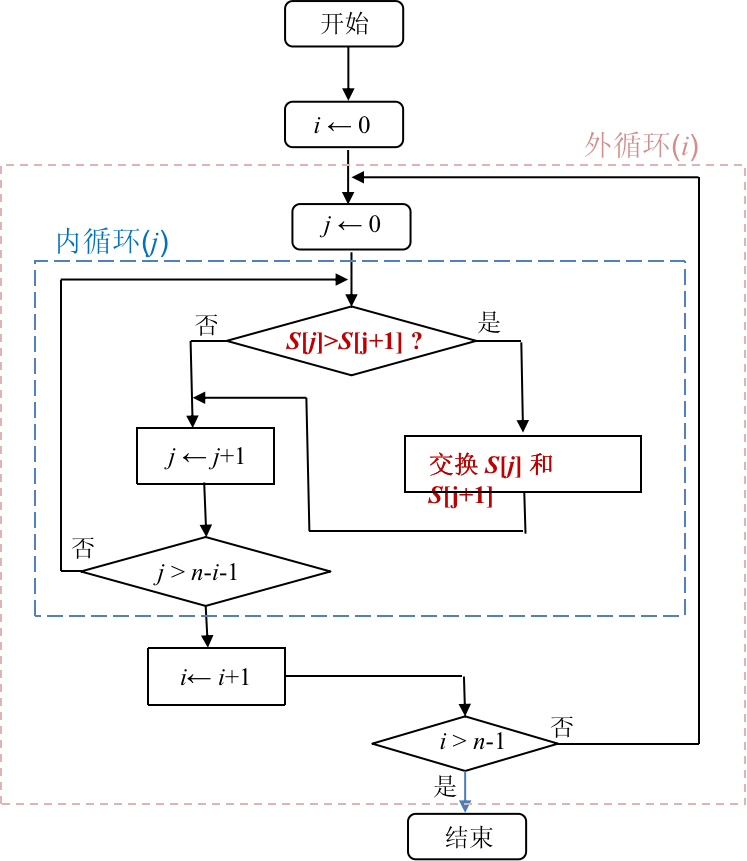
\includegraphics[scale=0.5]{2-prop-logic/figs/bubble-sort}
	\caption{冒泡排序的一个实现方法(流程图)}
	\label{fig:bub-sor}
\end{figure}


我们可以把内循环同样抽象成一个问题, 将一个(子)序列中的最大元素放到该子序列位置地址最大的地方(可以认为最后方). 那么对于它, 我们应该如何定义循环不变量? 

每次$i$循环开始前,序列 $S$ 中地址最高的 $i$ 个位置(除 $i=0$ 外, 即$S[n-i]$ 到 $S[n-1]$) 包含 $S$ 中前 $i$ 个最大的元素, 且已从小到大排好序; 序列中其它位置上的元素即 $S$ 中其它 $n-i$ 个元素. 

下面按照如下的三个方法归纳: 

\begin{itemize}
	\item 当$i=0$, 显然;
	\item 如果当 $i=k>0$ 时上述命题成立, 即 $k$ 循环开始前,  $S$ 中最大的 $k$ 个元素已被置换到 $S[n-k]$ 到 $S[n-1]$ ; 在 $k$ 循环中,指针 $j$ 从位置$0$扫描到位置$n-k-1$, 并将此范围内最大元素置换到$S[n-k-1]$. 则当$i=k+1$时, $S$ 中最大的 $k+1$个元素被排好序, 放置在 $S[n-(k+1)]$ 到 $S[n-1]$;
	\item 当 $i=n$, 算法终止, 即$n$循环(未执行)前,$n$ 个 $S$ 中的元素排好序, 并放置在 $S[0]$ 到 $S[n-1]$ 的位置上. 
 

\end{itemize}

\begin{bonus}
	在第一章里面我么说TRM里面有一条跳转指令, 为什么现在我们没有详细介绍goto指令, 并且绝大多数语言(除了C,C++)都没有了goto呢?
\end{bonus}

\begin{pas}
	\begin{center}
		\large \textbf{Go To Statement Considered Harmful(Cropped)}
	\end{center}
	\begin{center}
		E.W. Dijkstra\\
		from Communications of the ACM, Vol. 11, No. 3, March 1968, pp. 147-148
	\end{center}
	My first remark is that, although the programmer's activity ends when he has constructed a correct program, the process taking place under control of his program is the true subject matter of his activity, for it is this process that has to accomplish the desired effect; it is this process that in its dynamic behavior has to satisfy the desired specifications. Yet, once the program has been made, the ``making'' of the corresponding process is delegated to the machine.
	
	My second remark is that our intellectual powers are rather geared to master static relations and that our powers to visualize processes evolving in time are relatively poorly developed. For that reason we should do (as wise programmers aware of our limitations) our utmost to shorten the conceptual gap between the static program and the dynamic process, to make the correspondence between the program (spread out in text space) and the process (spread out in time) as trivial as possible.
	
	......
	
	The unbridled use of the go to statement has an immediate consequence that it becomes terribly hard to find a meaningful set of coordinates in which to describe the process progress. Usually, people take into account as well the values of some well chosen variables, but this is out of the question because it is relative to the progress that the meaning of these values is to be understood! With the go to statement one can, of course, still describe the progress uniquely by a counter counting the number of actions performed since program start (viz. a kind of normalized clock). The difficulty is that such a coordinate, although unique, is utterly unhelpful. In such a coordinate system it becomes an extremely complicated affair to define all those points of progress where, say, n equals the number of persons in the room minus one!

The go to statement as it stands is just too primitive; it is too much an invitation to make a mess of one's program. One can regard and appreciate the clauses considered as bridling its use. I do not claim that the clauses mentioned are exhaustive in the sense that they will satisfy all needs, but whatever clauses are suggested (e.g. abortion clauses) they should satisfy the requirement that a programmer independent coordinate system can be maintained to describe the process in a helpful and manageable way.

......

In [2] Guiseppe Jacopini seems to have proved the (logical) superfluousness of the go to statement. The exercise to translate an arbitrary flow diagram more or less mechanically into a jump-less one, however, is not to be recommended. Then the resulting flow diagram cannot be expected to be more transparent than the original one.


	
\end{pas}
 
\section{继续理解子过程和递归}

\subsection*{子过程}

在程序变的更加复杂的时候, 程序就会变得像面条一样难以驾驭. 这时候, 如果工程文件十分的大, 那么我们很可能会在这种情况下迷失. 比如写的一个C文件, 如果把所有的函数展开, 得到的一个难以阅读的文件. 可以用下面的命令得到一份. 

\begin{lstlisting}[language=sh]
	gcc your_file_name.c -S
\end{lstlisting}

之后文件夹下面就有一些.s文件了. 这是把C语言展开为了最基本的指令序列的结果. 可见, 当问题规模变得复杂的时候, 我们必须让复用重复的部分更加容易. 

比如, 我们要对一个句子里面含有``money''的词语计数, 我们可以有如下的算法. 

% TODO: 增加算法的图示和代码. 

\begin{bonus}
	所以, 用子过程有什么好处? 
\end{bonus}

事实上, 定义了子过程, 我们很多时候可以自己调用自己. 这对我们人类编写程序的时候是大有裨益的. 


\subsection*{递归}

在第一章我们用小纸条和老师以及作业本说明了什么是递归. 在这一节我们提供更多的例子. 


\begin{prob}[Hanoi塔问题]
 
\end{prob}

















